\section{Introduction}
One of the many reasons of the success of the Black-Scholes model (\citeauthor{black1973pricing}, \citeyear{black1973pricing}) is the existence of a one-to-one correspondence between the price $C(K,T)$ of an European call option with strike $K$ and time-to-maturity $T$ and the volatility $\sigma$ of the geometric Brownian motion modelling the dynamics of the underlying asset price $(S_t)_{t\ge0}$ provided that $(S_0-Ke^{-f_T T})^+ < C(K,T) < S_0$ ($f_T$ is the continuously compounded forward rate for the time-to-maturity $T$) which is guaranteed by absence of arbitrage opportunities. When this condition is satisfied, the unique parameter $\sigma$ satisfying $C_{BS}(K,T,\sigma)=C(K,T)$, where $C_{BS}$ denotes the Black-Scholes call option price, is called the implied volatility of the call option. By the put-call parity, the implied volatility of the put option is equal to the one of the call option with same time-to-maturity and strike. Although the implied volatility does not add any new information with respect to the option price, it is commonly used to quote option prices on the markets mainly because it allows to easily compare the value of two options with different underlying assets while the option price heavily depends on the underlying asset price level, making the comparison more difficult. If the Black-Scholes model was an accurate description of financial markets, the implied volatility should be the same for all options on a given asset regardless of the time-to-maturity and the strike. The computation of the implied volatility from market option prices shows that the implied volatility actually depends on the time-to-maturity and the strike which invalidates the Black-Scholes model. The so-called implied volatility surface (IVS) $(K,T)\mapsto \sigma_{BS}(K,T)$ permits to fully describe the option prices on a given asset. \\

It is also well-known that the level and the shape of the IVS varies with time. To be able to jointly model the time evolution of the IVS and the underlying asset price is key for applications covering asset allocation, risk management and hedging. First, such a model allows to backtest or study the P\&L distribution of an investment stragegy involving options and the underlying asset. One can think for example of the strategy consisting in buying a stock and a put of strike $K_1$ and selling a put of strike $K_2$ with $K_2<K_1$ but with same maturity (this is called a put spread). This strategy protects the investor against a drop in the underlying asset price down to the $K_2$ threshold in exchange to a lower premium in comparison to just buying a put of strike $K_1$. By extension, the modelling of the IVS and the underlying asset price makes it possible to optimize an asset allocation strategy involving options. Another application relates to the design and the backtesting of hedging strategies for financial products (e.g. volatility swaps, options on the VIX, etc.) having a volatility risk which is measured by the Black-Scholes vega. To complete this non-exhaustive list, let us finally mention that an IVS-underlying model can also be useful in the insurance industry for:
\begin{enumerate}
    \item computing the equity volatility distribution over a one-year horizon to estimate the capital requirement within Solvency II internal models and
    \item  assessing the time value of options and guarantees within insurance contracts and analyzing the underlying hedging strategies of long-term life insurance contracts embedding path-dependent options. 
\end{enumerate}
\subsection{Literature review}
Inspired by the market models of \cite{heath1992bond} and \cite{brace1997market} for the interest rates term structure, \cite{ledoit1998relative} and \cite{schonbucher1999marketmodel} independently proposed a modelling framework for the joint dynamics of the IVS and the underlying asset price where both are solutions of stochastic differential equations (SDEs) with the drift and volatility coefficients functions of the time, the time-to-maturity and the strike or moneyness variables only. In particular, no-arbitrage conditions on the drift are derived to guarantee the absence of arbitrage opportunities under the risk-neutral probability. A similar approach is adopted by \cite{brace2001market}. More empirical studies include the papers from \cite{skiadopoulos2000dynamics} and \cite{fengler2003dynamics}. The former applies a principal component analysis (PCA) to historical implied volatilities grouped in three time-to-maturity buckets and identifies two factors explaining 78\% of the smiles variation while the latter applies a common PCA and identifies three factors explaining more than 98\% of the variations. To deal with the fact that the study of the dynamics of the IVS is a three-dimensional problem (time, time-to-maturity and strike), \cite{cont2002dynamics} use a Karhunen-Loève decomposition instead of a PCA. They show that the dynamics of IVSs can be well summarized by three orthogonal factors which can be interpreted as the level, the orientation (i.e. a positive shock of this factor increases the volatilities of out-of-the-money calls while decreasing those of out-of-the-money puts) and the convexity of the surface. The associated principal components exhibit persistence (i.e. autocorrelation) and mean reversion close to the one of an $AR(1)$ process. Therefore, Cont and da Fonseca suggest to model each of the principal components as an Ornstein-Uhlenbeck process. \cite{cont2002stochastic} extend this model by specifying the dynamics of the underlying asset price which shares noise terms with the dynamics of the IVS allowing in particular to account for the correlation between the underlying price and the volatility surface level. A second extension, developed by \cite{cont2022simulation}, allows limiting the number of scenarios with static arbitrages by resampling from a given set of IVSs scenarios using smaller weights for scenarios with arbitrages. Another way to address this modelling problem in the literature is to resort to parametric or semi-parametric factors models, see e.g. \cite{hafner2005factor}, \cite{fengler2007semiparametric} or \cite{francois2023joint}. More recently, machine learning techniques such as GANs or neural SDEs have also been used to generate realistic simulations of implied volatility surfaces, see e.g. \cite{wiese2019deep}, \cite{cohen2021arbitrage}, \cite{zhang2023} and \cite{choudhary2024}. Finally, let us mention the paper of \cite{morel2024path} who introduced the so-called Path Shadowing Monte Carlo method which, combined with a statistical model of prices, allows to make state-of-the-art predictions of option smiles using only the distribution of the price process.  \\

In this paper, we develop a new joint model of the IVS and the underlying asset price. Instead of specifying the IVS as the solution of a given SDE or as a linear combination of several factors (whether parametric, semi-parametric or non-parametric), we propose to consider a parameterization of the IVS whose parameters evolution depends on the path of the underlying asset price. The chosen parameterization is the celebrated SSVI parameterization of \cite{gatheral2014arbitrage} that is known to well reproduce observed IVSs and guarantees the absence of static arbitrage under mild conditions. This modelling paradigm consisting in making dynamic the parameters of a model fitting market data at some point in time is similar to the one of \cite{carmon2011tangent} who developed a very general mathematical framework for designing consistent dynamic market models. In \cite{carmona2017levy}, the authors provide a practical implementation of this framework for IVSs allowing to simulate IVSs that are free of both static and dynamic arbitrage. Moreover, they use these simulations of IVSs to find the portfolio with smallest variance for a portfolio consisting of $n$ options of same maturity but different strikes. In the same vein, \cite{bloch2021deep} used an SVI model whose parameters are stochastic processes to model the dynamics of the entire IVS. A convolutional LSTM (Long Short-Term Memory) neural network is used to learn the joint dynamics of these parameters and the underlying forward price. There is one main difference between our approach and the ones of these papers and the literature in general. In our approach, we introduce an explicit modelling of the impact of the underlying asset price onto the level and the shape of the IVS in the spirit of \cite{guyon2022volatility} who focus on volatility indices and realized volatility (hence not on vanilla options implied volatilities). Indeed, in the above literature, the dependence structure between the IVS and the underlying asset price is generally captured through simple assumptions such as a Gaussian copula, common noise terms or using the short-term implied volatility as a term in the underlying asset stochastic volatility dynamics. Moreover, we model the underlying price using the path-dependent volatility framework of \cite{guyon2022volatility} which exhibits high statistical consistency and captures multiple historical stylized facts (leverage effect, volatility clustering, weak and strong Zumbach effects). Before giving more details on our approach, we find useful to dedicate a section to Guyon and Lekeufack's main results.

\subsection{Guyon and Lekeufack's path-dependent volatility model}\label{sec:pdv_model}
\cite{guyon2022volatility} showed that the level of the volatility of major equity indices is essentially explained by the past variations of these equity indices, or in other words, they showed that volatility is mostly path-dependent. To be more specific, they consider two measures of the volatility: the value of an implied volatility index such as the VIX and an estimator of the realized volatility over one day using intraday observations of the equity index. We recall that an implied volatility index is a measure of the expected future variance\footnote{Note that the VIX can also be interpreted as the implied volatility of the 30-days log-contract $-\frac{2}{\tau}\log \frac{S_{t+\tau}}{F_t^{t+\tau}}$ on the S\&P 500 index ($F_t^{t+\tau}$ is the forward price at time $t$ with maturity $t+\tau$). } of a given underlying index (for example the S\&P 500 for the VIX) at a given horizon $T$. Mathematically, the expected future variance writes $\mathbb{E}\left[\frac{1}{T}\int_0^T \sigma_t^2 dt \right]$ where $\sigma$ is the instantaneous volatility of the underlying index and $\mathbb{E}$ here denotes the expectation under the risk-neutral probability. The expected future variance can be estimated from the prices of traded calls and puts on the underlying index using the \cite{carr2001formula} formula. We refer for example to the documentation of the VIX (\citeauthor{vixwp}, \citeyear{vixwp}) or the VSTOXX (\citeauthor{vstoxxwp}, \citeyear{vstoxxwp}) for more details. Note that Guyon and Lekeufack only use short-term implied volatility indices (the horizon $T$ is below 30 days) since they are interested in the modelling of the instantaneous volatility. Let us now introduce the model that they calibrate for both measures of volatility. Let $(S_t)_{t\ge 0}$ be the price process of an equity index and $\text{Volatility}_t$ be one of the two above-mentioned measures of volatility. The Path-Dependent Volatility (PDV) model from the empirical study of \cite{guyon2022volatility} writes as follows:
\begin{equation}\label{eq:guyon_model}
    \text{Volatility}_t = \beta_0+\beta_1 R_{1,t} + \beta_2\Sigma_t.
\end{equation}
The features $R_{1,t}$ and $\Sigma_t$ are defined on a time grid $(t_i)_{i\in \mathbb{N}}$ as follows:
\begin{itemize}
    \item $R_{1,t}$ is a trend feature given by:
\begin{equation}\label{eq:r1_formula}
    R_{1,t} = \sum_{t_i \le t} K_1(t-t_i) r_{t_i}
\end{equation}
where $r_{t_i}= (S_{t_i}-S_{t_{i-1}})/S_{t_{i-1}}$ and $K_1:\mathbb{R}_+\rightarrow \mathbb{R}_+$ is a decreasing kernel weighting the past returns. Since the value of $\beta_1$ estimated by \cite{guyon2022volatility} is negative, this feature allows to capture the leverage effect, i.e. the fact that volatility tends to rise when prices fall.
\item $\Sigma_t$ is an activity or volatility feature given by:
\begin{equation}\label{eq:sigma_formula}
    \Sigma_t = \sqrt{\sum_{t_i \le t} K_2(t-t_i) r_{t_i}^2}
\end{equation}
where $K_2$ also is a decreasing kernel. Since the value of $\beta_2$ estimated by \cite{guyon2022volatility} is positive, this feature allows to capture the volatility clustering phenomenon, i.e. the fact that periods of large volatility tend to be followed by periods of large volatility, and periods of small volatility tend to be followed by periods of small volatility. 
\end{itemize}
In order to capture both the short and long memory of volatility, they propose a time-shifted power law (TSPL) for the two kernels $K_1$ and $K_2$:
\begin{equation}\label{eq:tspl_kernel}
    K_j(\tau) = \frac{Z_{\alpha_j,\delta_j}}{(\tau+\delta_j)^{\alpha_j}},\quad j=1,2,
\end{equation}
with $Z_{\alpha_j,\delta_j}$ the normalization constant such that $\sum_{t-C\le t_i \le t} K_j(t-t_i)\Delta  = 1$ where $\Delta  = 1/252$ (business days frequency) and $C$ is a hyperparameter (called the cut-off lag later in the paper) controlling at which point the sums in $R_1$ and $\Sigma$ are truncated. Note that it is not clear whether the volatility obtained using Equation (\ref{eq:guyon_model}) is positive. For time-continuous versions of the features $R_1$ and $\Sigma$, sufficient conditions guaranteeing the volatility's positivity have been given by \cite{guyon2022volatility} and \cite{nutz2024} in the case of two exponential kernels, i.e. $K_j(\tau) = \lambda_j e^{-\lambda_j\tau}$ for $j\in\{1,2\}$ and by \cite{andres2024existence} for more general choices of $K_2$. However, the framework of the latter does not cover the case when $K_1$ is a TSPL kernel or a convex combination of two exponential kernels, i.e. $K_1(\tau)=\theta \lambda_{1}e^{-\lambda_{1}\tau}+(1-\theta)\lambda_{2}e^{-\lambda_{2}\tau}$, which is a good approximation of TSPL kernels proposed by \citeauthor{guyon2022volatility}. Thus, the volatility's positivity is still an open question for these choices of kernels. Let us nevertheless mention that \citeauthor{guyon2022volatility} observe only non-negative volatilities in their simulations when using two convex combinations of two exponential kernels and "realistic parameter values".   \\

In order to measure to which extent the two features of the PDV model allow to explain the variations of the volatility, they use the $R^2$ score:
\begin{equation}\label{eq:r2}
    R^2(y,\hat{y}) = 1-\frac{\sum_{i=1}^{n}(y_i-\hat{y}_i)^2}{\sum_{i=1}^{n}(y_i-\bar{y}_n)^2}
\end{equation}
where $y=(y_i)_{1\le i\le n}$ are the observed data, $\hat{y}= (\hat{y}_i)_{1\le i\le n}$ are the predicted data and $\bar{y}_n=\frac{1}{n}\sum_{i=1}^{n}y_i$. When they calibrate the PDV model on implied volatility indices data, they obtain $R^2$ scores over tested indices that are above 87\% on the train set (January 1, 2000 to December 31, 2018) and above 80\% on the test set (January 1, 2019 to May 15, 2022), which shows that the PDV model explains a large part of the variability observed in the volatility dynamics. In Figure \ref{fig:guyon_graphs}, we reproduce two graphs from their paper that indicate quite clearly the linear relationship between the two features and the VIX. When calibrated on realized volatility data, the performance of the PDV model is reduced: the $R^2$ score is about 70\% on the train set and 60\% on the test set. 
% \begin{figure}
%     \centering
%     \begin{subfigure}{0.4\textwidth}
%         \centering
%         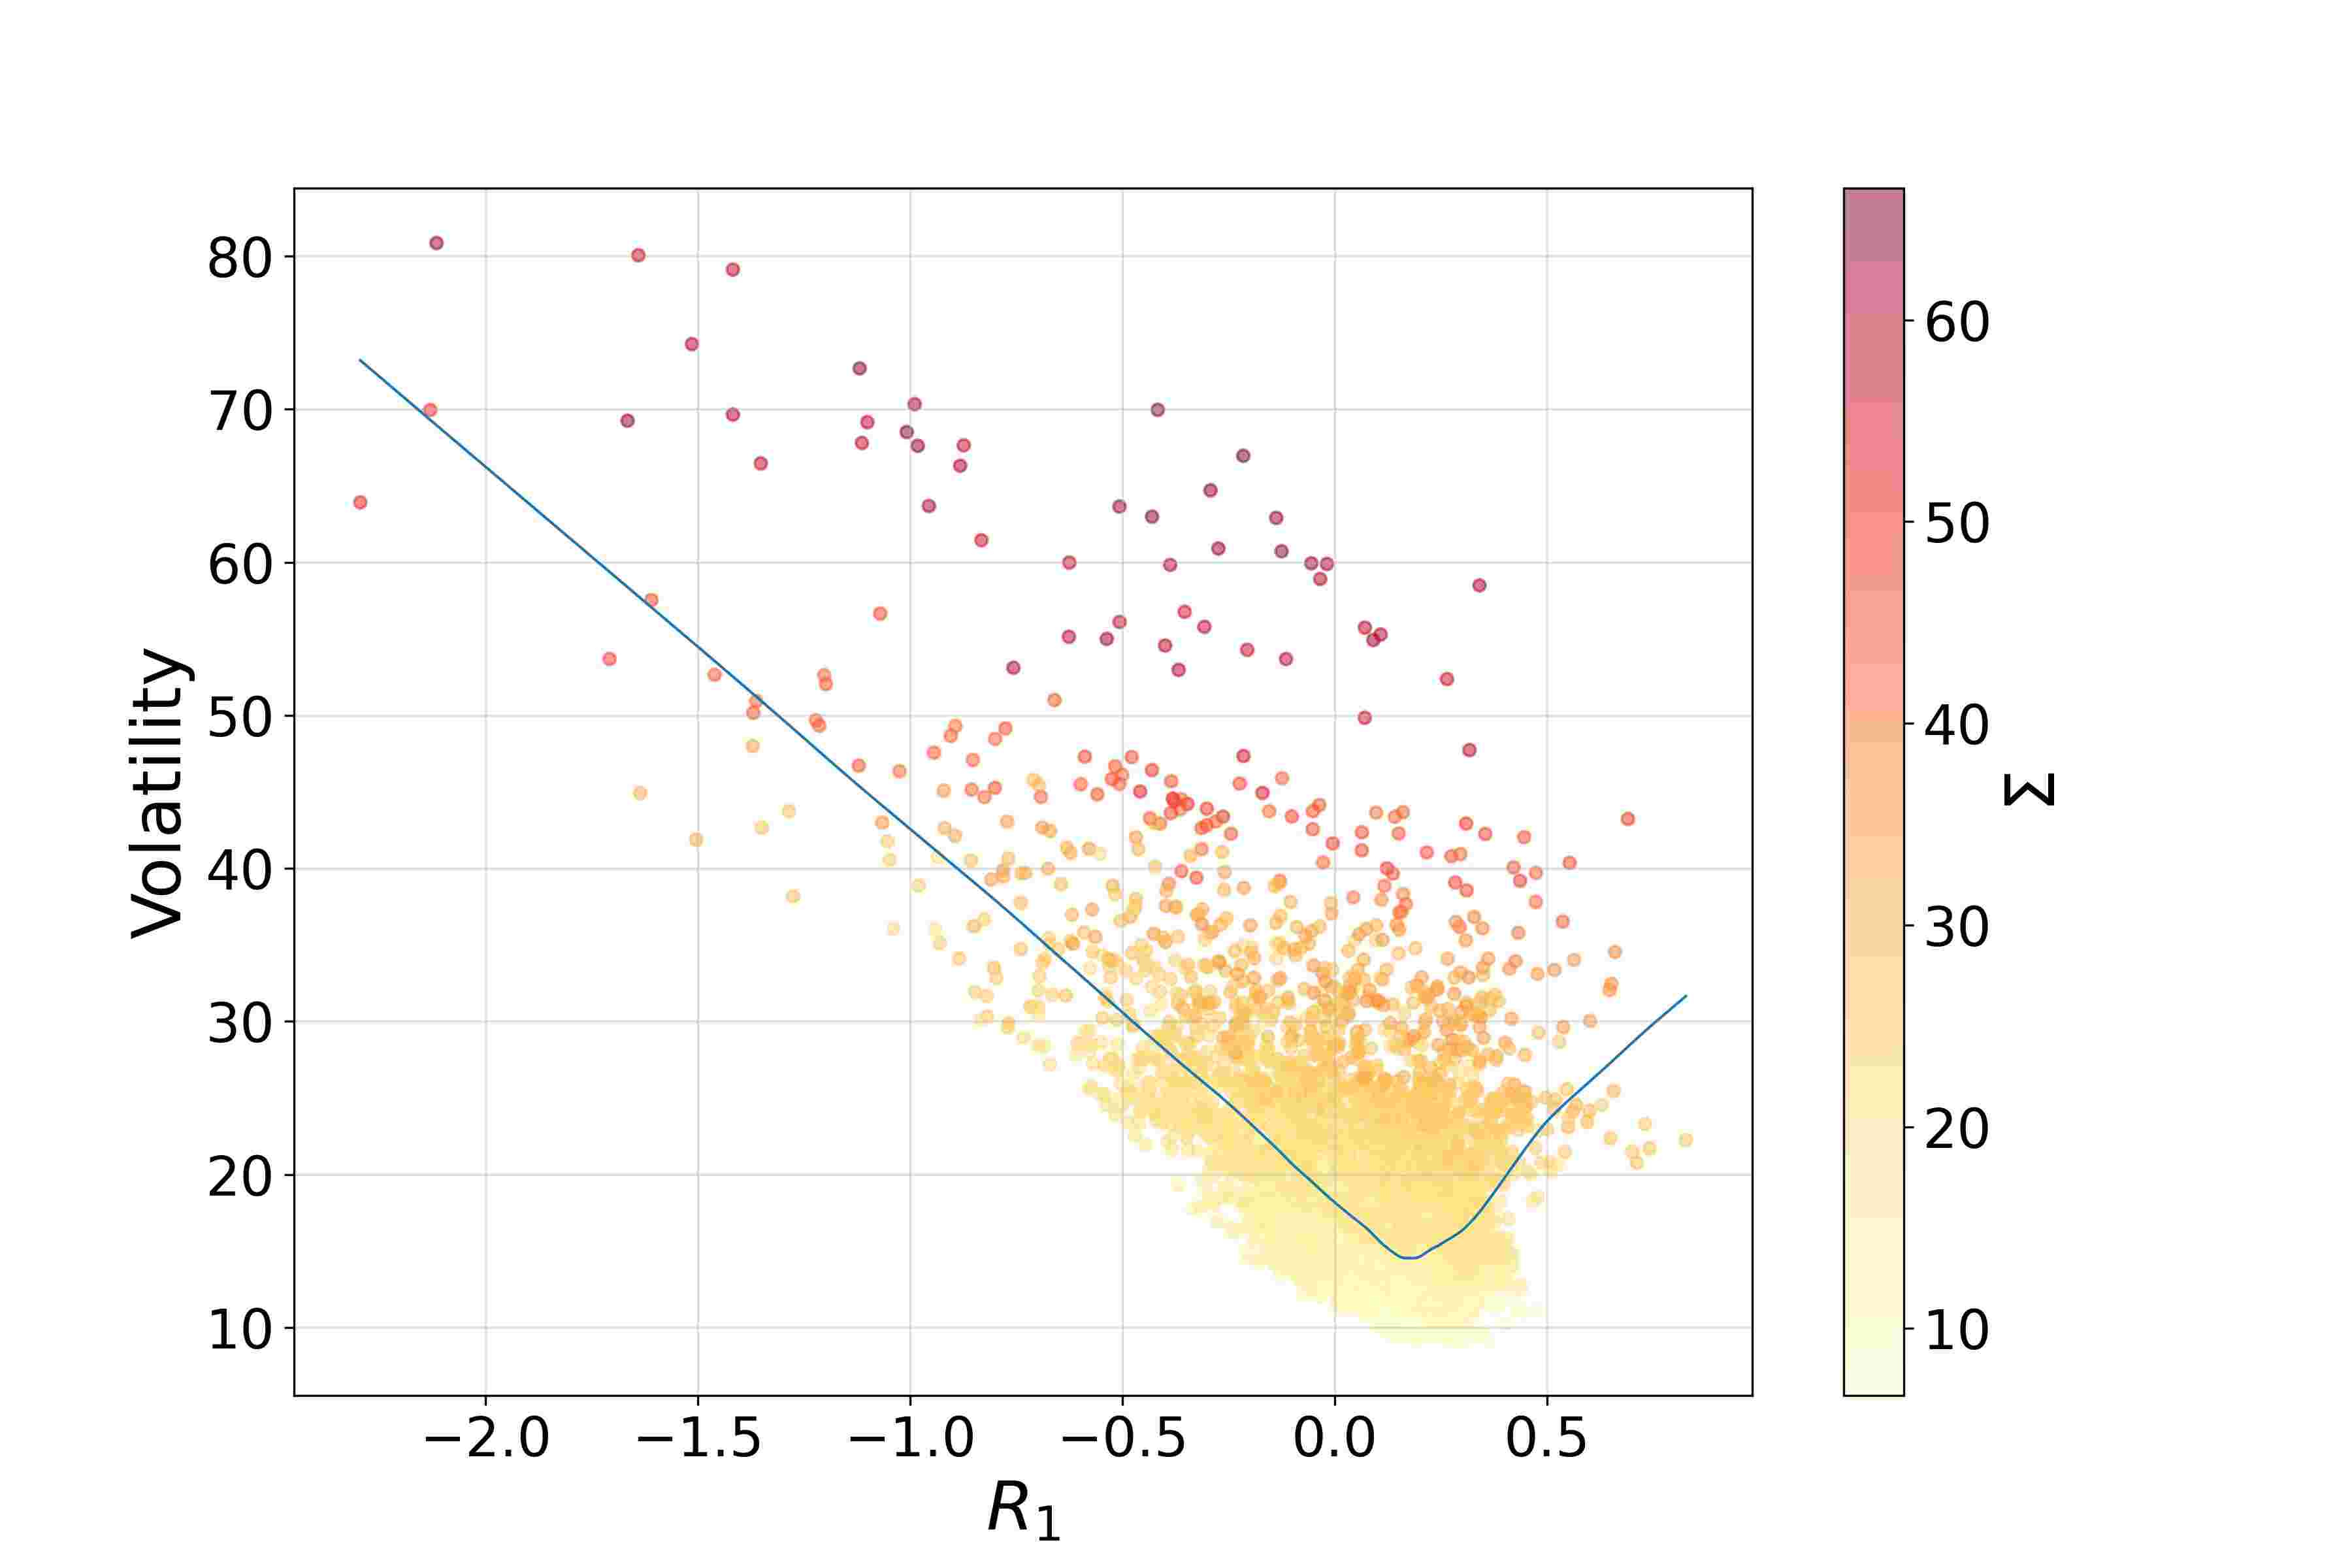
\includegraphics[width=\linewidth]{VIX_R1.jpg}
%         \caption{VIX vs $R_1$}
%     \end{subfigure}
%     \begin{subfigure}{0.4\textwidth}
%         \centering
%         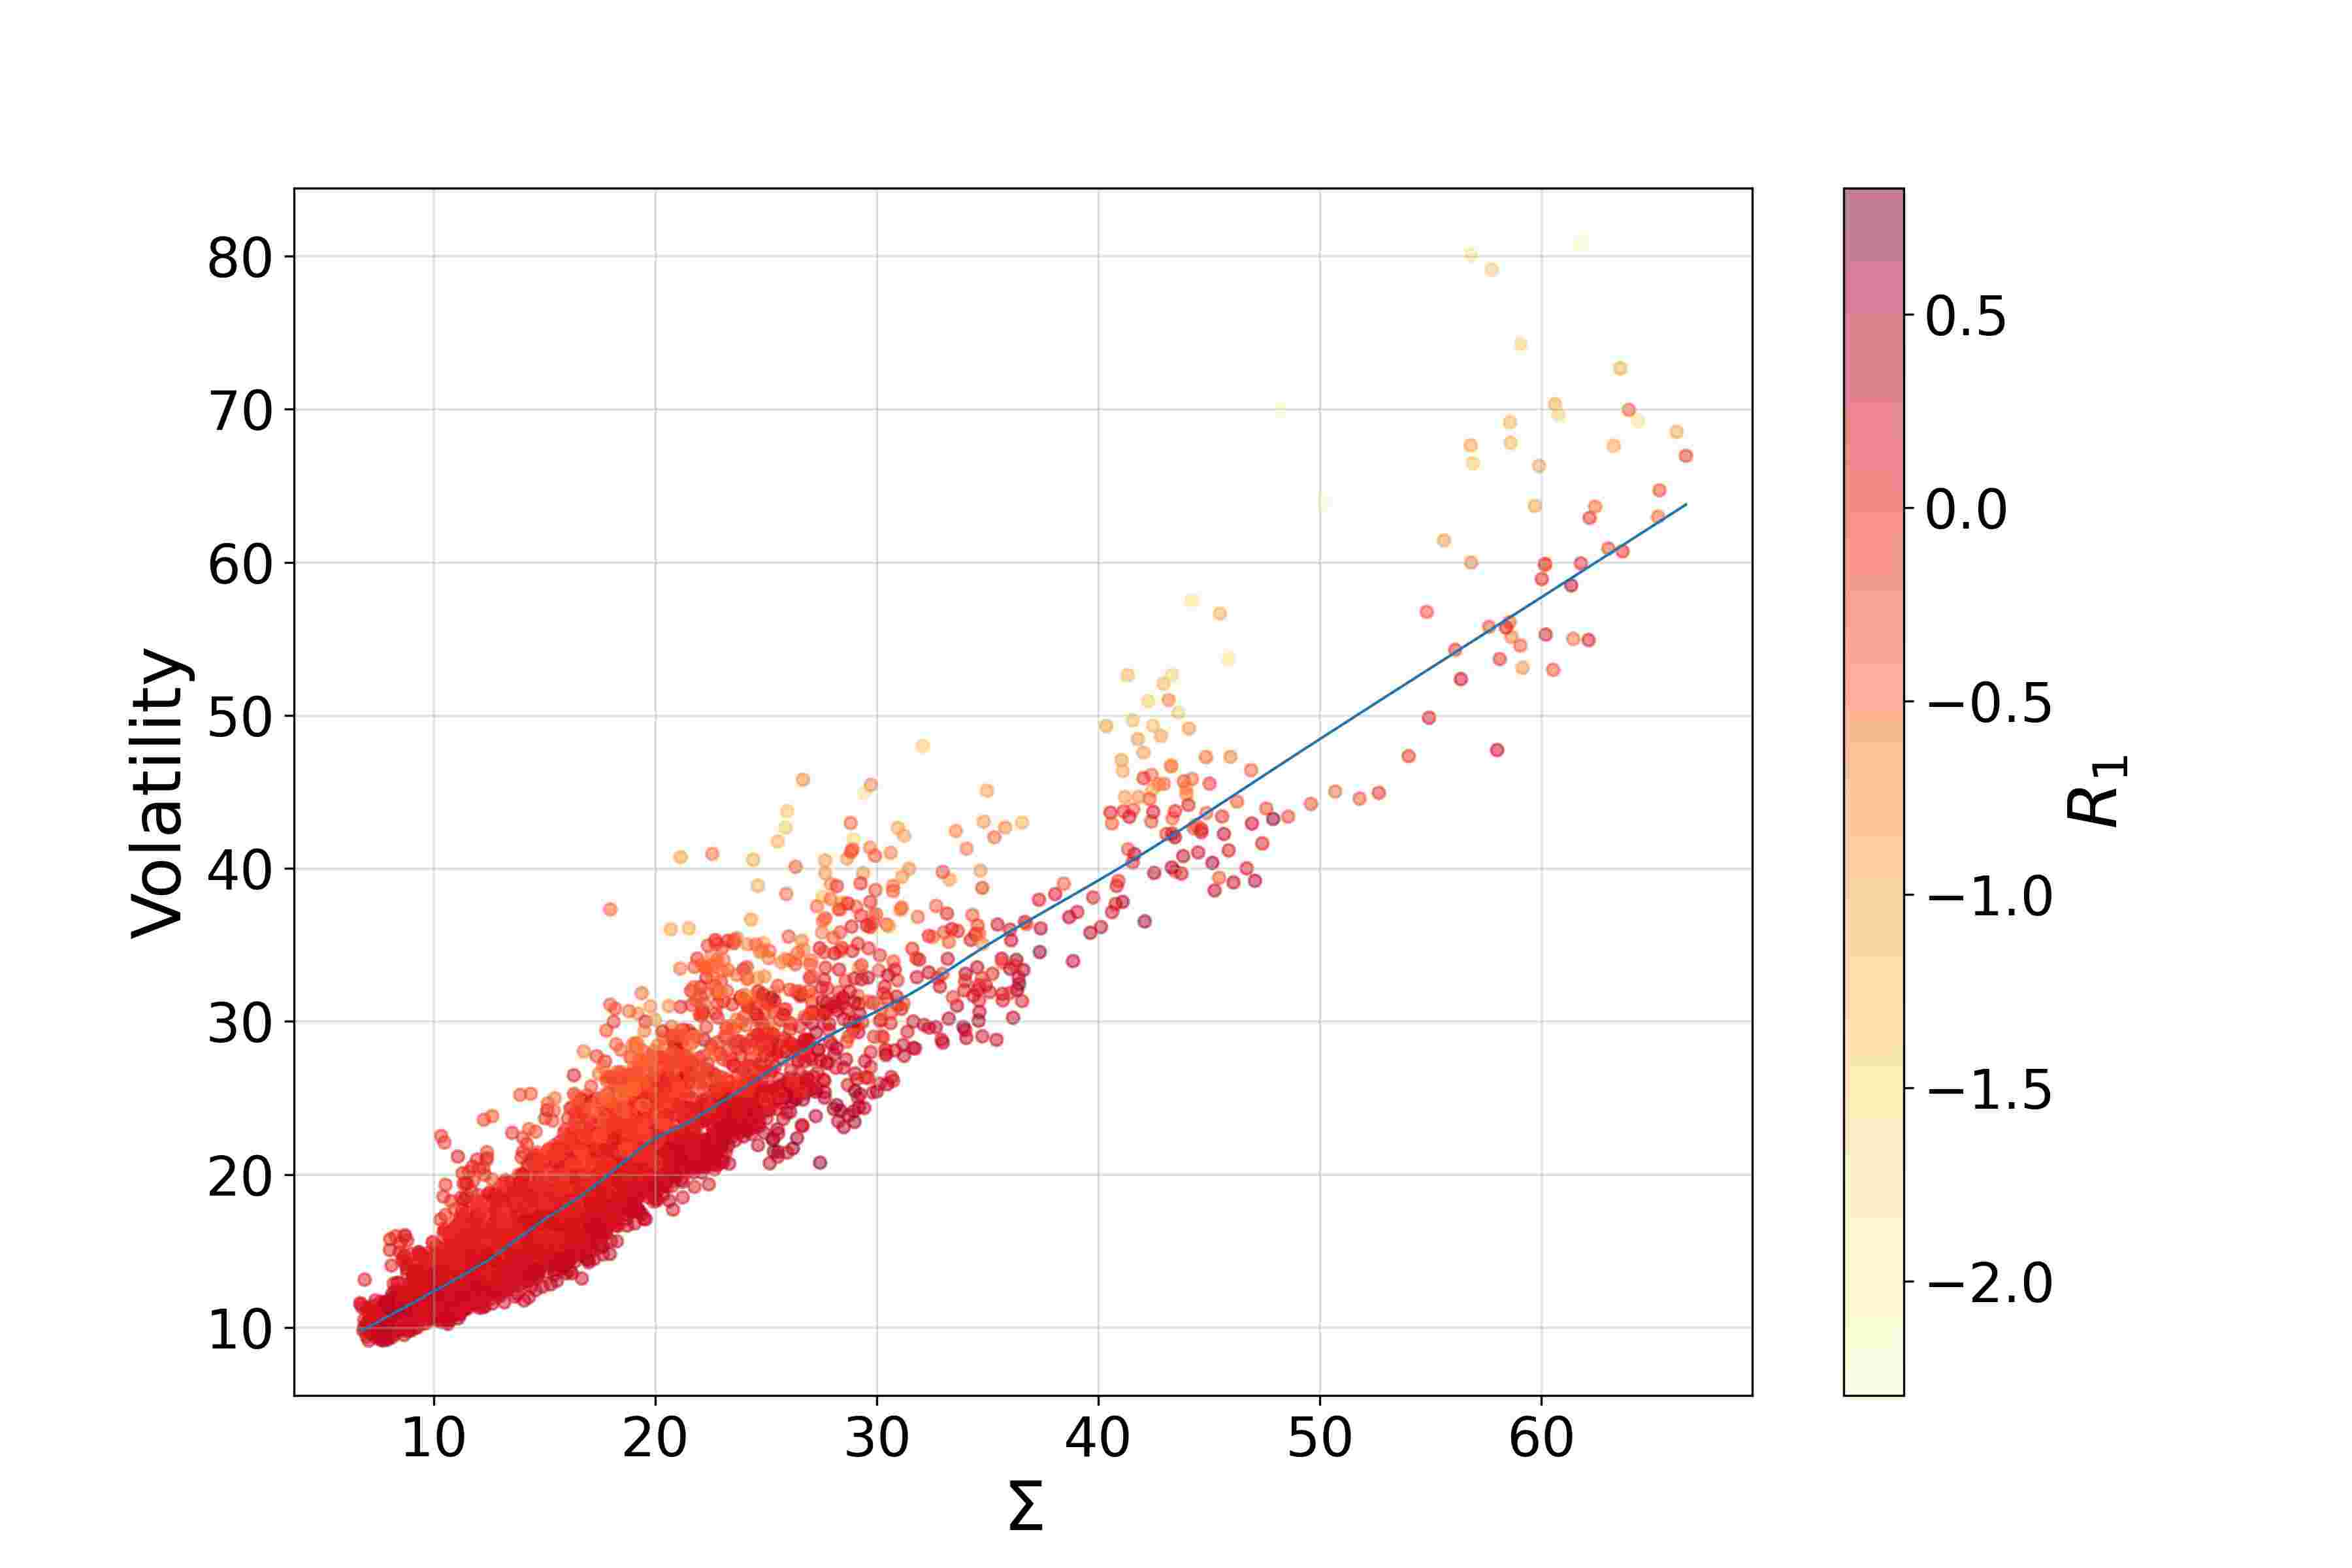
\includegraphics[width=\linewidth]{VIX_Sigma.jpg}
%         \caption{VIX vs $\Sigma$}
%     \end{subfigure}
%     \caption{Values of the VIX against values of the features $R_1$ and $\Sigma$ on the train set. The blue line represents $\mathbb{E}[Y\mid X]$ (obtained by a locally weighted scatterplot smoothing) when displaying $Y$ vs $X$. }
%     \label{fig:guyon_graphs}
% \end{figure}
\begin{figure}
    \centering
    \subfigure[VIX vs $R_1$]{ 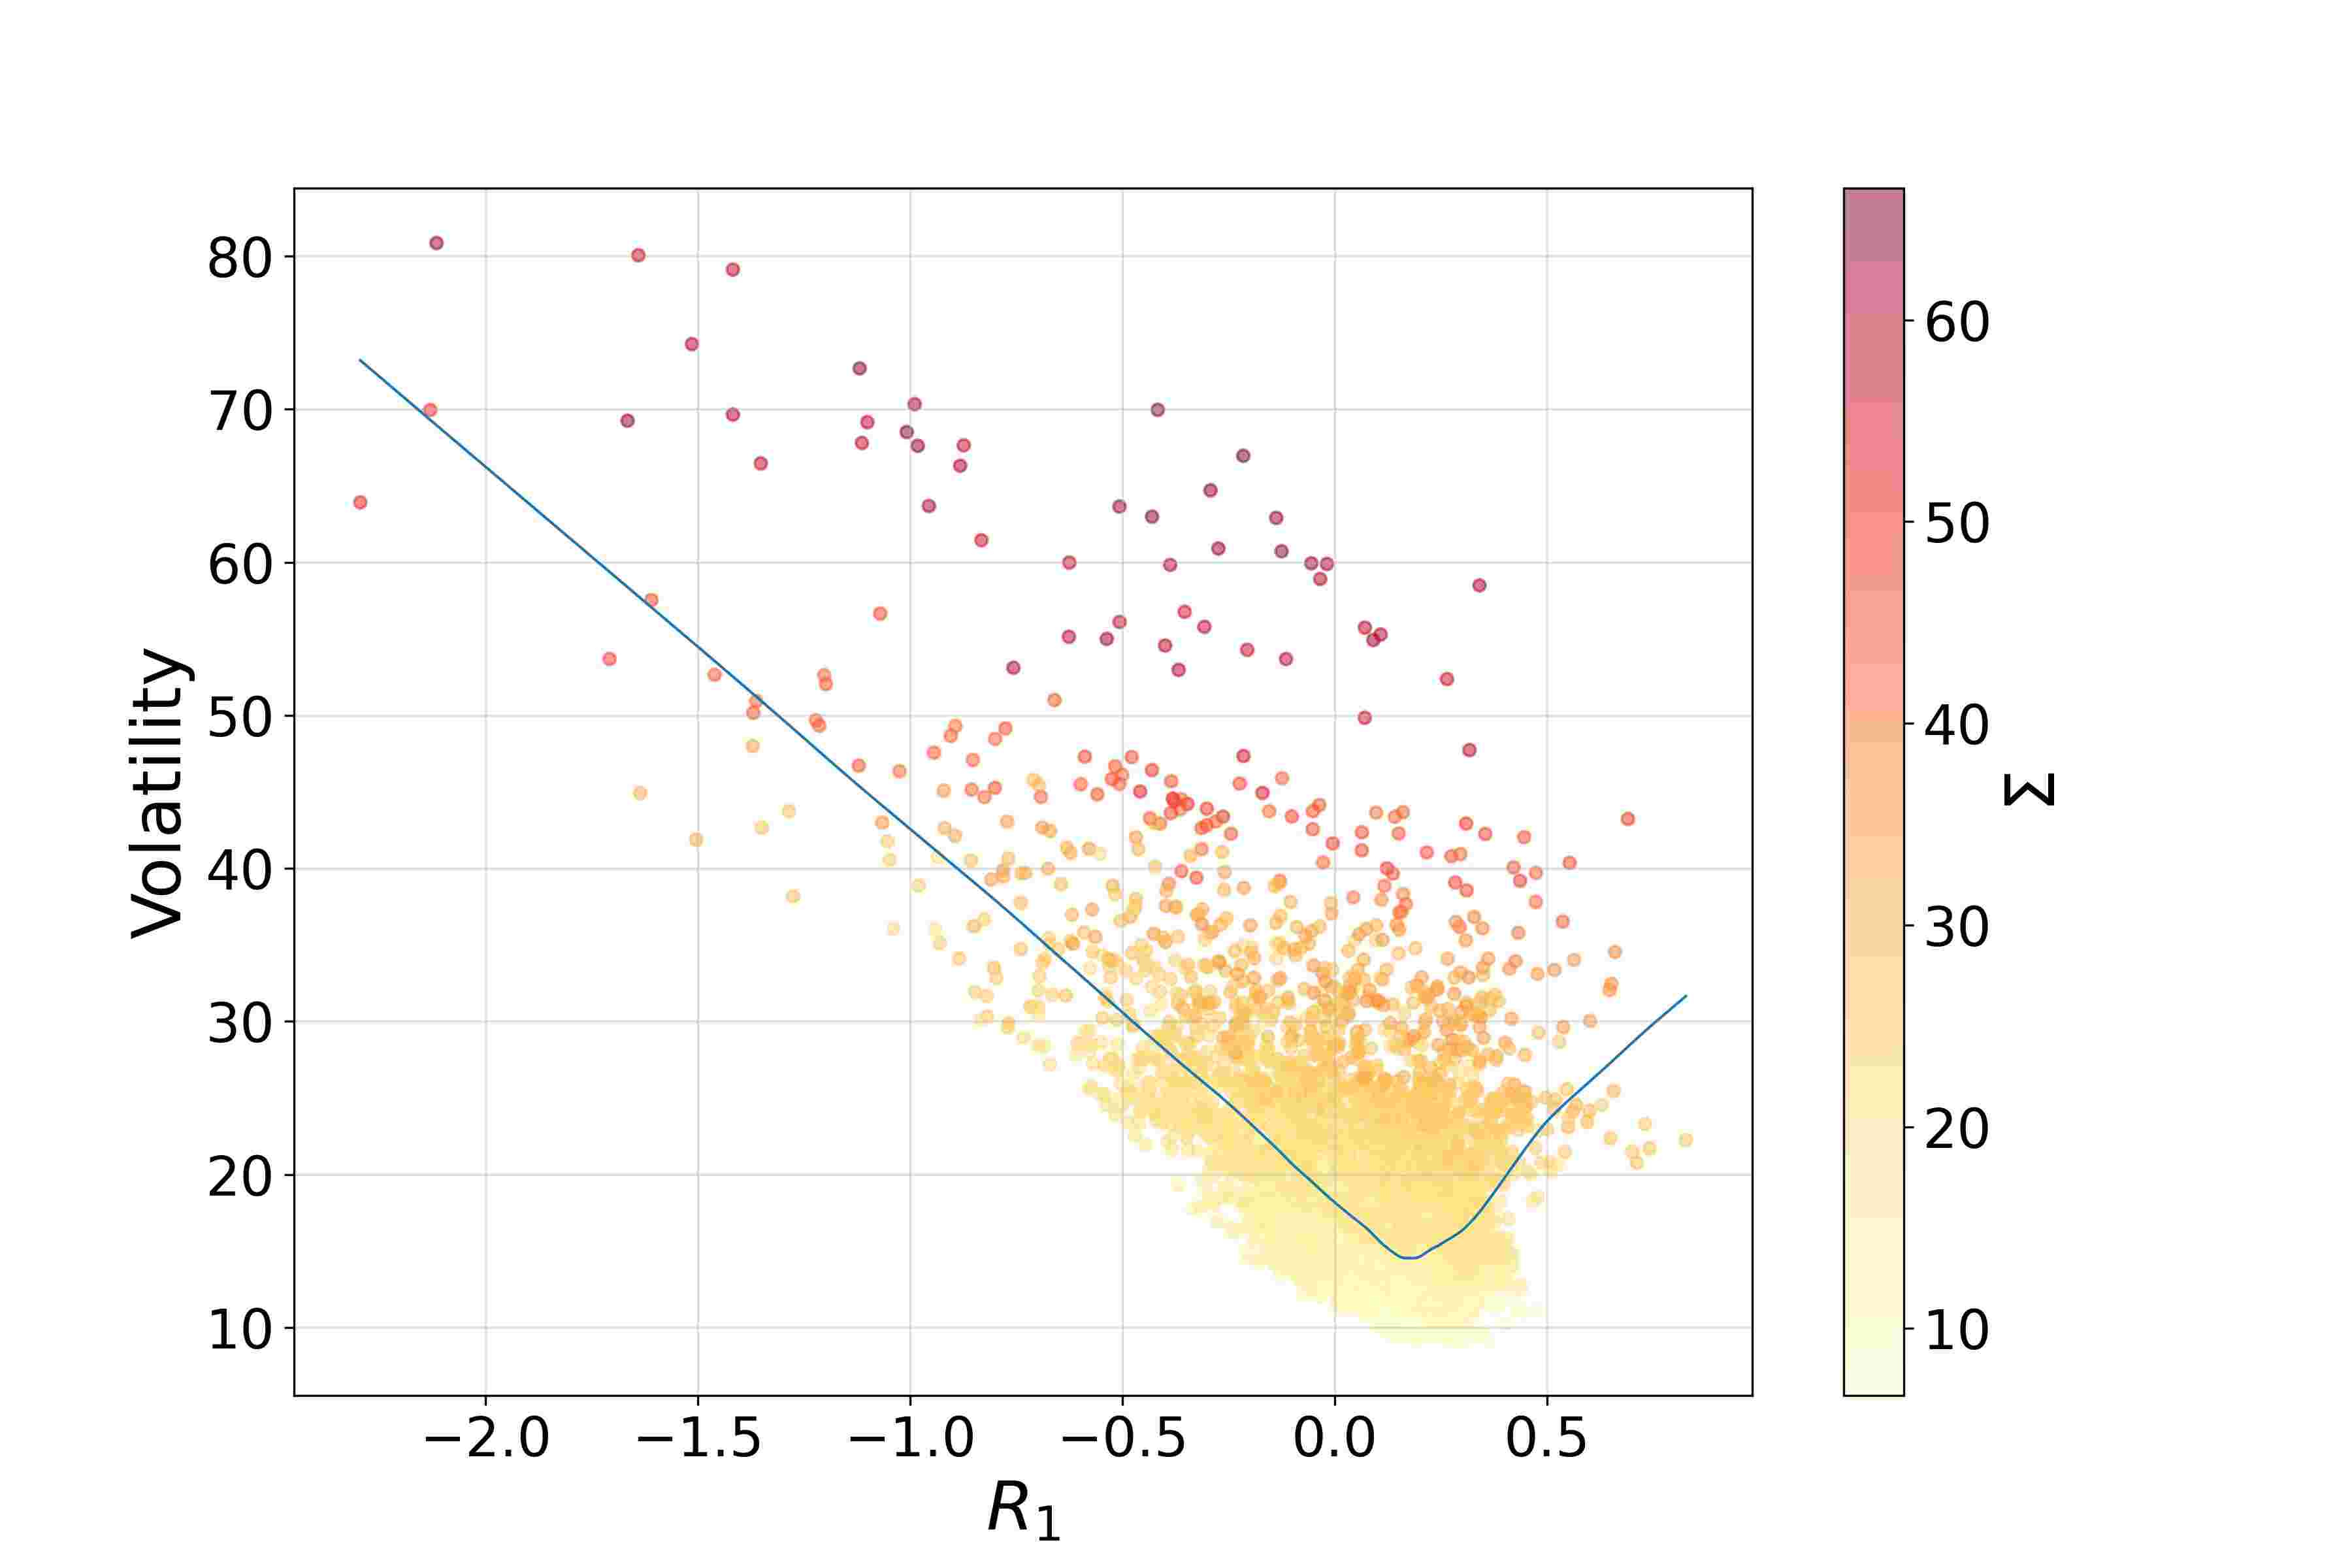
\includegraphics[width=0.45\linewidth]{VIX_R1.jpg}}
    \subfigure[VIX vs $\Sigma$]{ 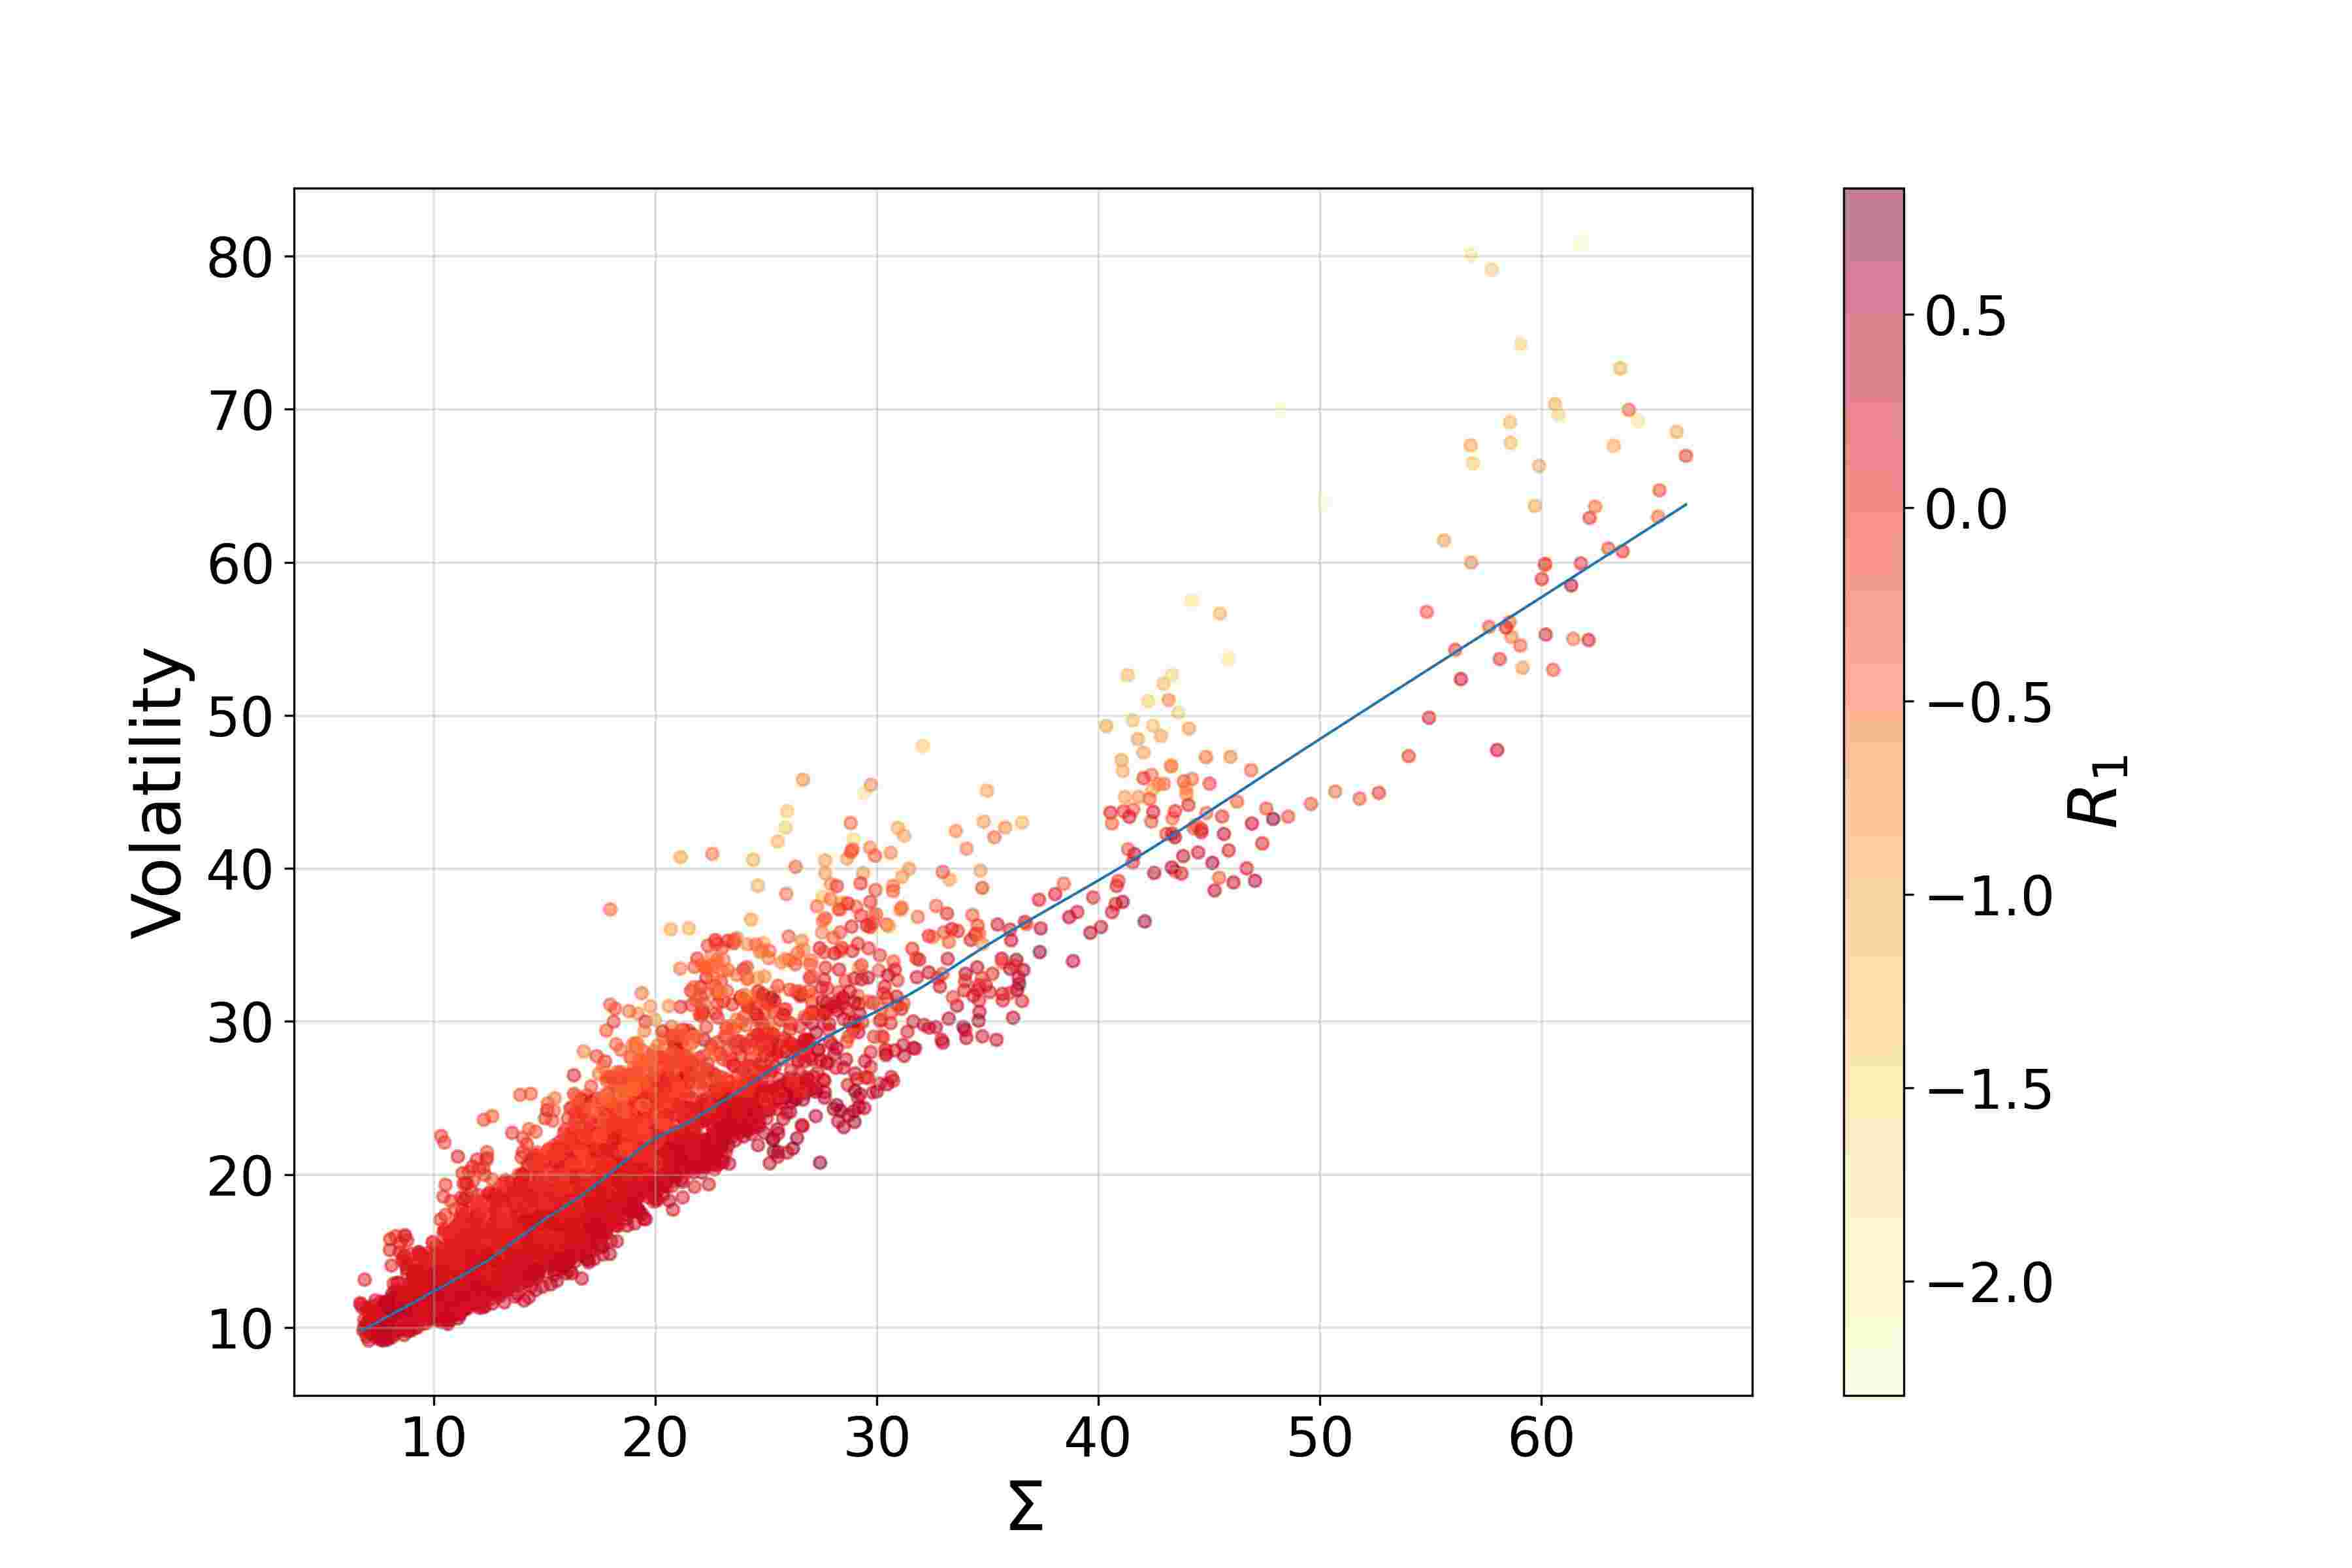
\includegraphics[width=0.45\linewidth]{VIX_Sigma.jpg}}
    \caption{Values of the VIX against values of the features $R_1$ and $\Sigma$ on the train set. The blue line represents $\mathbb{E}[Y\mid X]$ (obtained by a locally weighted scatterplot smoothing) when displaying $Y$ vs $X$.}
    \label{fig:guyon_graphs}
\end{figure}

\subsection{Contributions}
The first contribution of the present paper is an empirical study of the dependence of implied volatility on the past movements of the underlying asset price for options on the S\&P 500 and options on the Euro Stoxx 50. This empirical study is inspired by the one of \cite{guyon2022volatility} but there are several differences. First and foremost, we work on vanilla implied volatility instead of implied volatility indices: the former is directly determined by supply and demand while the latter is determined as linear combinations of prices of calls and puts covering the liquid strikes and the two time-to-maturities that are the closest to 30 days. Both are therefore close only if we consider implied volatilities of 1-month time-to-maturity options. Since we consider time-to-maturities up to 24 months, our study can be seen as an extension of the one of \cite{guyon2022volatility}. Second, we analyze the influence of the cut-off lag of the kernel on the performance of the PDV model. Finally, we add a regularization term in the calibration of the model and study its impact. Our study also differs from the numerous studies in the literature around implied volatility forecasting. For example, \cite{bakshi2000call} focus mostly on the frequency with which call (resp. put) prices move in the same direction (resp. opposite direction) as the underlying asset price but they do not try to exhibit a functional relationship between the two and they do not use the past path of the underlying asset price. \cite{cao2020} train a neural network using as input features the S\&P 500 daily return, the time-to-maturity and the Black-Scholes delta to predict the variation in the S\&P 500 implied volatility surface (in a second step, they also use the level of the VIX). Their model provides better predictions than a benchmark model and is consistent with the negative correlation between the asset returns and the implied volatility variations that was already documented in the literature. However, this paper does not explore additional explanatory features beyond the asset price return the day before the prediction. Finally, \cite{wen2024implied} explore how daily implied volatilities up to 20 days in the past allow predicting future implied volatilities. They obtain out-of-sample $R^2$ scores up to 80\% and conclude that implied volatility is (almost) path-dependent. The study we present differs from this one in that we focus solely on the dependence of implied volatility with respect to the past path of the asset price and not to the past path of implied volatilities. Moreover, we use a time window larger than 20 days in our study and we use TSPL kernels to weight the past instead of considering one separate weight for each lagged value of the implied volatility.  \\

The second contribution is to propose a parsimonious version of the Surface Stochastic Volatility Inspired (SSVI) parameterization (\citeauthor{gatheral2014arbitrage}, \citeyear{gatheral2014arbitrage}) of the IVS which relies only on four parameters and provides a reasonable replication of the market IVSs for a wide range of dates. This parsimonious SSVI parameterization is free of static arbitrage provided that a simple inequality constraint involving two parameters is satisfied. We also show that the two parameters governing the ATM implied volatility curve as a function of the time-to-maturity can be well explained by the past path of the underlying asset price. \\

Our final contribution is to introduce a new model for the joint dynamics of the underlying asset price and the implied volatility surface allowing to perform Monte Carlo simulations under the real-world probability. This model is obtained by specifying the time evolution of the four parameters of the parsimonious SSVI parameterization for the IVS and combining it with a variant of the PDV model of \cite{guyon2022volatility} for the underlying price. The dynamics of the two parameters governing the ATM implied volatility curve contains a functional dependence on the past path of the underlying price allowing to embed in the model the feedback effect that we observe on historical data. Moreover, the residuals of these two parameters are modelled using Ornstein-Uhlenbeck processes and the two others parameters of the parsimonious SSVI parameterization are modelled using Jacobi processes. Together with the model specification, we also provide a calibration methodology for all the parameters that are involved in the dynamics. Ultimately, we show through several metrics that the IVSs simulated with our model are highly realistic. \\

This paper is organized as follows: in Section \ref{sec:empirical_study}, we start by the empirical study of the dependence of implied volatility on the past movements of the underlying asset price. Then, we present the SSVI parameterization and its parsimonious version as well as some calibration results in Section \ref{sec:svi}. Finally, Section \ref{sec:pdv_ssvi} is dedicated to the introduction of our new path-dependent SSVI model for simulating implied volatility surfaces and the underlying asset price. 

% Défauts modèle de Cont: on modélise le log donc j'ai l'impression que c'est pas stationnaire
% Article de Parent:
% - étude de l'autocorrélation des résidus et plus globalement du besoin d'ajouter du bruit exogène -> cf calcul de la vol sur données simulées sans ajout d'une source de bruit exogène + illustrations trajectoires 

% Insister sur le fait que l'on étend les résultats de Julien